\chapter{Marco teórico} \label{chap:marco}                                                              % ##   2.

Antes de prosseguirmos com o desenrolar deste trabalho, é adequado que primeiro definamos alguns conceitos para o melhor entendimento do trabalho como um todo. Iniciaremos com a definição do \hyperref[sec:termos]{Problema de \textit{timetabling}}, suas subdivisões, \hyperref[ssec:desafios]{suas complexidades} e \hyperref[ssec:erros]{possíveis errosna gestão das informações}. Em seguida, abordaremos os \hyperref[sec:resolucao]{métodos de resolução} para o problema, nos baseando em compilados de informações sobre os trabalhos anteriores. Especifica-se também como que se dá o \hyperref[sec:anteriores]{Problema de \textit{Timetabling na UENF (PTT-UENF)}}, com base nos trabalhos anteriores. Por fim, são apresentadas diversas \hyperref[sec:teorias]{estratégias de solução baseadas na otimização}, que serão utilizadas conceitualmente durante o desenvolvimento deste trabalho.

% O Problema de Programação de Horários (Timetabling Problem) é um problema de grande relevância e amplamente estudado na área de Pesquisa Operacional. Um número significativo de trabalhos sobre esse problema foi publicado nos últimos anos e conferências regulares discutem o tema no meio científico [Splinder2010].
% Sânya
% O Problema de Programação de Horário Escolar pode ser generalizado como o escalonamento semanal das aulas em uma escola sem que professores e alunos tenham mais de uma aula ao mesmo tempo (estudantes são agrupados em turmas com os mesmos planos de aula). Já o Problema de Programação de Horário de Disciplinas em Universidades como o escalonamento semestral das aulas de um conjunto de disciplinas de uma universidade de modo a evitar colisão de horários (estudantes geralmente são considerados individualmente) [Paim__2010].
% Sânya

% Existem algumas ferramentas comerciais que prometem a geração automatizada de grades de horários, entretanto, sua utilização é pouco frequente uma vez que este tipo de problema incorre em necessidades específicas de um determinado curso, em detrimento das soluções genéricas existentes
% F. Vieira & H. Macedo, Scientia Plena 7, 039901 (2011) 

% O school timetabling possui uma quantidade de recursos menor, pois uma turma já possui uma sala especificada e seu grupo de alunos, em sua maioria, é predeterminado, o que faz com que a complexidade seja reduzida. Em problemas de course timetabling existe um grande conjunto de restrições: disciplinas de uma mesma turma podem ser alocadas em salas diferentes, cada disciplina é constituída por alunos de diversos cursos, professores possuem restrições de horário por desempenharem outras atividades na instituição, cada disciplina possui conjuntos de pré-requisitos que devem ser respeitados, entre outras.
% F. Vieira & H. Macedo, Scientia Plena 7, 039901 (2011) 

\section{Problema de \textit{timetabling}} \label{sec:termos}                                                        % ###  2.1

% Ao longo dos anos de desenvolvimento acadêmico, diversos assuntos vão se aprofundando e se tornando mais específicos, assim, os estudiosos acabam cunhando novos termos que o auxiliam a desvencilhar as novas áreas específicas das suas áreas originárias. Porém, existe o potencial de que haja um crescimento desestruturado destes novos termos, assim vários termos diferentes podem se referir a um mesmo conceito, enquanto que um mesmo termo pode se referir a vários conceitos diferentes de acordo com o autor.

Segundo \citeonline{Wren1996}, \textit{timetable} é definido como uma estrutura que mostra quando eventos ocorrerão, não havendo necessariamente a alocação de recursos. Vale ressaltar que este termo não tem seu uso limitado para os fins desta pesquisa, sendo também usado para problemas de alocação de enfermeiros, esportes, funcionários e transportes \cite{Arratia2021}. Entretanto, neste trabalho, abordaremos principalmente os termos relacionados ao que pode ser chamado de \textit{Educational Timetabling} (Ed-TT) \cite{Alencar2019}, que é o que tende a envolver um conjunto específico de recursos relacionados à educação.

\citeonline{Wren1996} também define os conceitos para \textit{class timetable}, \textit{university examination timetable} e \textit{university class timetable}, tendo relevância apenas o último, que considera a disponibilidade de professores e salas, a quantidade de alunos e os requisitos que determinada disciplina exige.

Assim como feito por \citeonline{Wren1996}, definiremos os conceitos dos termos que serão usados ao longo deste trabalho. Sendo assim, usaremos a definição do termo \textit{university class timetable} de forma simplificada, sendo chamada apenas de \textit{timetable}, ``grade horária'' ou ``tabela horária''.

% Sânya fala sobre International Timetabling Competition

Aqui, visto que uma solução final envolverá várias dimensões (Professores $\times$ Disciplinas $\times$ Sala $\times$ Alunos $\times$ Horários $\times$ Dias), consideraremos \textit{timetable} como esse pacote de valores distribuídos em uma só estrutura. Para que esses valores sejam distribuídos, daremos o nome de \textbf{alocação} ao ato de criar qualquer relação entre as dimensões. Como a relação de horários e dias será considerada fixa, a \textbf{alocação} se referirá à atribuição como a de professores a disciplinas, disciplinas a salas, disciplinas a um determinado padrão de dias e horários, etc.

Para que esta alocação ocorra, é necessário atender a certos critérios, e aí entra o ``problema de organização de grade horária'', também chamado de \textit{timetabling problem}. Esta é uma subcategoria do \textbf{problema de otimização de agendamento} (\textit{scheduling Optimization Problem}) \cite{Alencar2019} que por sua vez é definido por \citeonline{Wren1996} como sendo:

\begin{quote}\footnotesize
  Resolver problemas práticos relacionados à alocação, sujeito a restrições, de recursos a objetos sendo colocados no espaço-tempo, usando ou desenvolvendo quaisquer ferramentas que possam ser apropriadas. Os problemas irão frequentemente se relacionar à satisfação de certos objetivos. \cite{Wren1996}
\end{quote}

Outro termo relevante a se pontuar são as \textit{hard and soft constraints} que podemos chamar de restrições rígidas e flexíveis. \citeonline{Alencar2019} as definem dizendo que as restrições rígidas são de atendimento obrigatório para que a solução seja considerada viável, enquanto as restrições flexíveis são opcionais, mas convenientes para melhorar a qualidade da solução obtida.

Ambos os tipos de restrições são importantes para a resolução do problema, e são altamente dependentes do contexto em que estão inseridas. Em determinada instituição de ensino. Por exemplo: uma restrição rígida onde uma disciplina não possa durar mais do que três horas pode ser considerada flexível em outra instituição. Sendo então, também dependente do contexto de cada instituição a definição das regras de viabilidade e inviabilidade de soluções.

Em seu trabalho, \citeonline{Souza2000} distingue entre viabilidade e otimalidade. Para ele, no primeiro caso, a solução do problema consiste basicamente em encontrar um conjunto de alocações tal que satisfaça a todas as restrições impostas. Já no segundo caso, após encontrar-se diversas soluções viáveis, busca-se dentre elas aquelas que melhor atendam às soluções flexíveis baseado em critérios de avaliação de uma função objetivo. \citeonline{Dunke2023} comentam que há algoritmos que consideram as restrições rígidas e flexíveis de forma simultânea, enquanto outros resolvem primeiro as restrições rígidas e depois as flexíveis.

Alguns outros termos similares a este campo de pesquisa encontrados na literatura são \textit{periodic event scheduling problem}, \textit{timetable scheduling}, \textit{class scheduling}, \textit{student scheduling}, \textit{university course timetabling}, dentre outros.

\subsection{Questões sobre a complexidade do problema} \label{ssec:desafios}                                                      % ###  2.3

% Apesar da vasta quantidade de trabalhos realizados na área do \textit{Timetabling Problem} segue sendo estudado como devida.

\citeonline{Murray2007} trazem a questão da modelagem como um dos maiores obstáculos. À medida em que a complexidade aumenta, se torna cada vez mais difícil desenvolver uma solução efetiva. Assim fazendo com que a solução para uma universidade possa não ter utilidade para outras, ou até mesmo não seja capaz de lidar com todos os problemas de uma mesma universidade.

Apesar do contrafluxo encontrado na resolução desse problema, \citeonline{Murray2007} citam que, apesar da complexidade, é sim possível desenvolver soluções que tenham uso prático, mesmo que não seja um processo fácil. As ferramentas existem e estão disponíveis. Restando então considerar e resolver as preocupações dos usuários às questões, visto que as técnicas de resolução já se encontram vastamente documentadas.

Com isso, entramos também no ramo da Interação Homem-Máquina, ramo abordado por \citeonline{Andre2018} que visaram em seu desenvolvimento a criação de uma interface focada no usuário. Assim minimizando o atrito na abordagem desse problema complexo. Também sendo área de enfoque de \citeonline{Alencar2019} em sua revisão literária

\subsection{Possíveis erros na gestão das informações} \label{ssec:erros}                                                    % ###  2.5

Dada a grande quantidade de variáveis interconectadas e as características específicas de cada instituição \cite{Miranda2012}, a organização destas informações buscando a melhor solução possível apresenta-se como um desafio. Principalmente se considerarmos que esta solução é, muitas vezes, procurada manualmente, estando também passível de erros humanos como ilustram a \autoref{fig:Academico} e \autoref{fig:CCT}.

\begin{MyCenteredFigure} \caption{Disciplina atribuída no sistema acadêmico à determinada hora e local} \label{fig:Academico}
  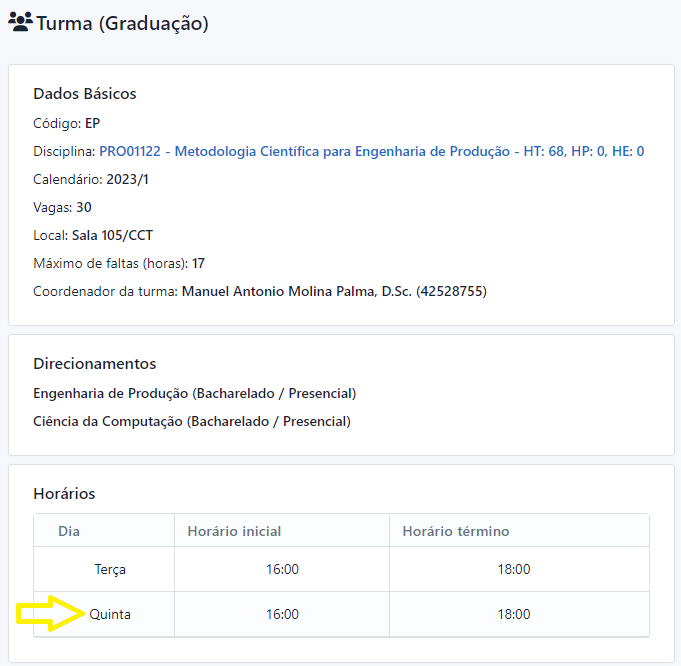
\includegraphics[width=0.8\textwidth]{files/img/2.02!2-marco/Metodologia-Quinta}
\end{MyCenteredFigure}

\begin{MyCenteredFigure} \caption{Falha de alocação na grade horária do CCT de 2023.1} \label{fig:CCT}
  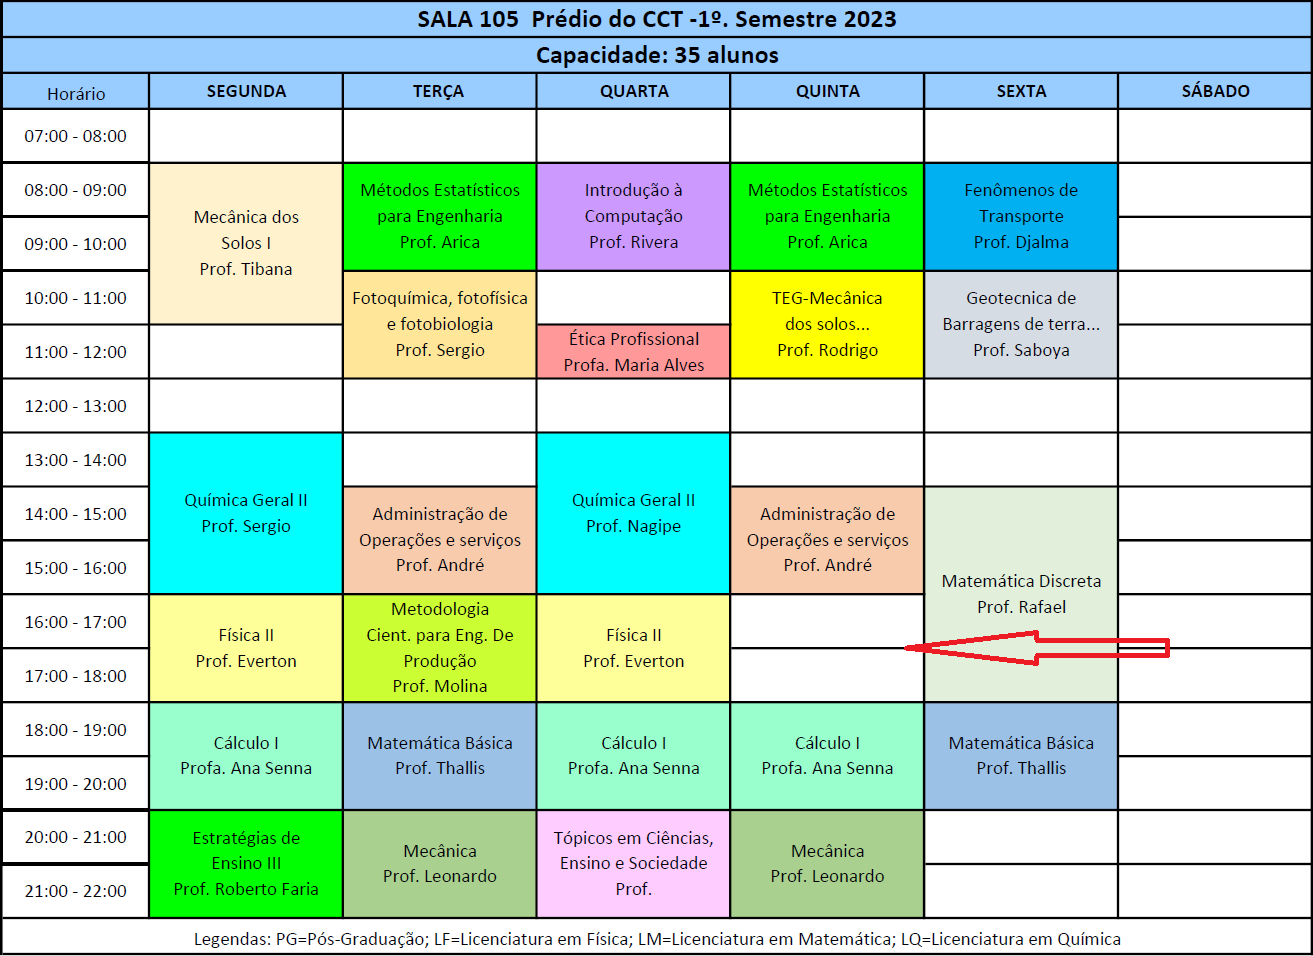
\includegraphics[width=0.8\textwidth]{files/img/2.02!2-marco/Aulas-CCT-105-2023_1}
\end{MyCenteredFigure}

Nestas imagens, fica exemplificado um dos possíveis problemas que podem ocorrer durante a criação de grades horárias, devido à falta de integração das informações em um sistema único. Situação essa que ocorre quando uma seção da universidade (o Sistema Acadêmico, ilustrado pela \autoref{fig:Academico}) aloca uma turma a uma determinada sala, outra seção da mesma instituição (o Centro de Ciência e Tecnologia, ilustrado pela \autoref{fig:CCT}) pode não estar ciente do mesmo, ou, mesmo estando ciente, pode acabar não delimitando aquela lacuna de tempo como ocupada, assim estando passível de uma segunda alocação naquele período de tempo naquela sala, assim gerando problemas.

\section{Métodos de resolução para o problema de \textit{timetabling}} \label{sec:resolucao}                                                    % ###  2.2

% - O problema de timetabling  a
%  - Origem                    a
%  - Repartições               a
%  - Escopo maior              a
%    - Scheduling              a
%  - Escopo menor              a
%    - Exam                    a
%    - Class                   a
% - TT
%  - Soluções
%  - Desafios
%  - Diversas formas de resolução
%    - Graph Coloring
%    - Heurísticas
%    - Metaheurísticas
%    - IA
%    - etc.
% - Visualização de informações
%  - Benefícios
%  - Motivações
%  - Relação com timetabling
% - Problema geral a ser resolvido
%  - Multi dimensionalidade
%    - Professores
%    - Alunos
%    - Salas
%    - Departamentos
%      - Preferências
%      - Concorrências
%  - Otimalidade
%  - Erros humanos
%  - Número de possibilidades
%  - Interface intuitiva e relevante é um desafio com poucos estudos nos últimos anos
% - Problemas específicos
%  - Regras específicas
%  - Prioridades diferentes
%  - estrutura organizacional semi-exclusiva

% Pesquisar posteriormente sobre imagens que ilustrem bem as diferentes sub categorias de scheduling

Existem diversas implementações já realizadas, utilizando uma miríade de métodos. Em seu trabalho, \citeonline{Miranda2012} informam sobre diversos sistemas baseados em computador para auxiliar na tarefa de agendamento. \citeonline{Miranda2012} também citam dois possíveis métodos de resolução, sendo eles o \textbf{modelo de programação inteira} e os \textbf{métodos heurísticos}.

Dada a variedade de publicações acadêmicas nessa área de estudo, alguns trabalhos buscaram condensar em forma de tabela as informações encontradas. A seguir, algumas das tabelas mais relevantes encontradas durante o estudo bibliográfico serão apresentadas em conjunto com uma breve descrição e análise sobre seu conteúdo.

Na \autoref{fig:Desenvolvimento}, \citeonline{Poulsen2012} traçam a relação entre os diversos autores, ano de sua publicação e seu país de origem com os dados encontrados em seus trabalhos quanto aos parâmetros utilizados na elaboração da grade horária, quão grandes eram cada um de seus parâmetros, quanto tempo foi necessário para achar uma solução e quais foram as técnicas utilizadas.

% Entender o que está dando errado aqui depois

\begin{CenteredFigure} \caption{Resumo de trabalhos, parâmetros, dimensões, tempo e técnicas.} \label{fig:Desenvolvimento}
  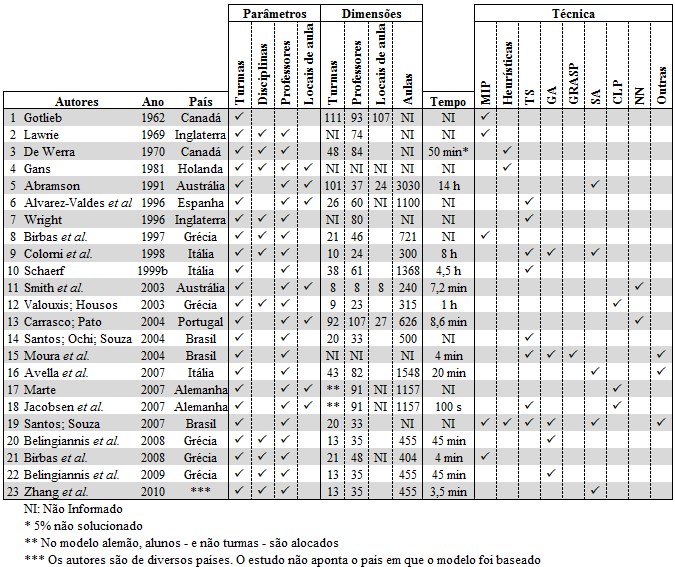
\includegraphics[width=\textwidth]{files/img/2.02!2-marco/Desenvolvimento}
  \legend{Fonte: \citeonline{Poulsen2012}}
\end{CenteredFigure}    % Desenvolvimento

Na \autoref{fig:University}, \citeonline{Arratia2021}, apresentam uma comparação similar à anterior, porém não separada em categorias, apenas categorizando entre verdadeiro e falso algumas características como alocação de salas, professores, nível institucional e método de solução exato ou aproximado.

\begin{CenteredFigure} \caption{Comparação entre artigos que solucionam o problema de grade horária} \label{fig:University}
  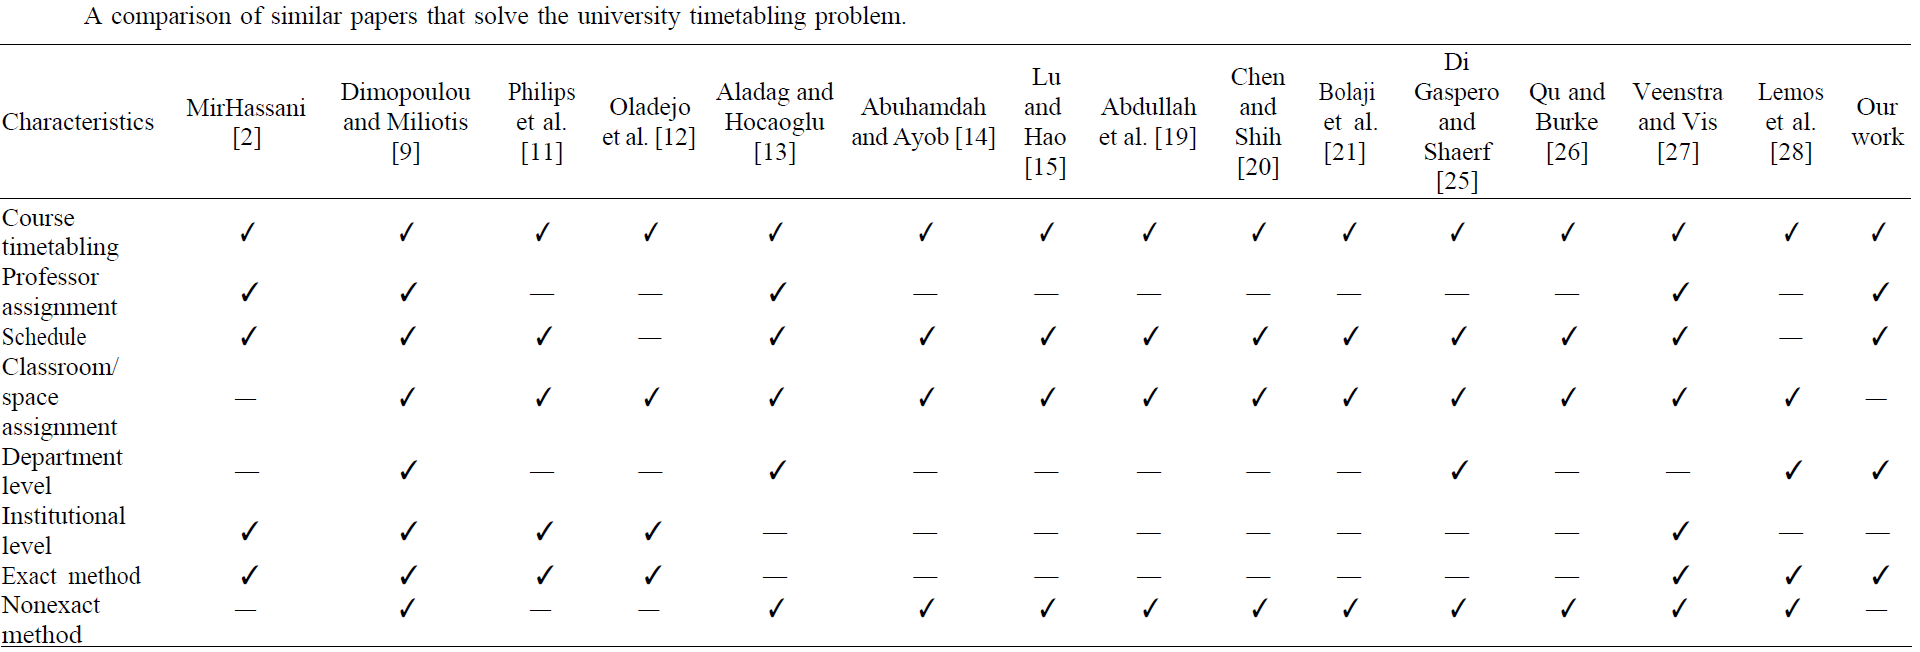
\includegraphics[width=\textwidth]{files/img/2.02!2-marco/University}
  \legend{Fonte: \citeonline{Arratia2021} - editado}
\end{CenteredFigure}    % University

Na \autoref{fig:Visualization}, \citeonline{Alencar2019} exploram uma categoria mais específica do problema, que é a característica da interatividade das interfaces desenvolvidas. Este apresenta características qualitativas quanto aos métodos, os dados dispostos, as técnicas de interação e o método utilizado para solucionar o problema de grade horária educacional. Nesta figura, os autores usam ``Y'' para simbolizar ``Sim'', ``N'' para ``Não'' e ``-'' para ``Inconclusivo''.

\begin{CenteredFigure} \caption{Análise de publicações aceitas} \label{fig:Visualization}
  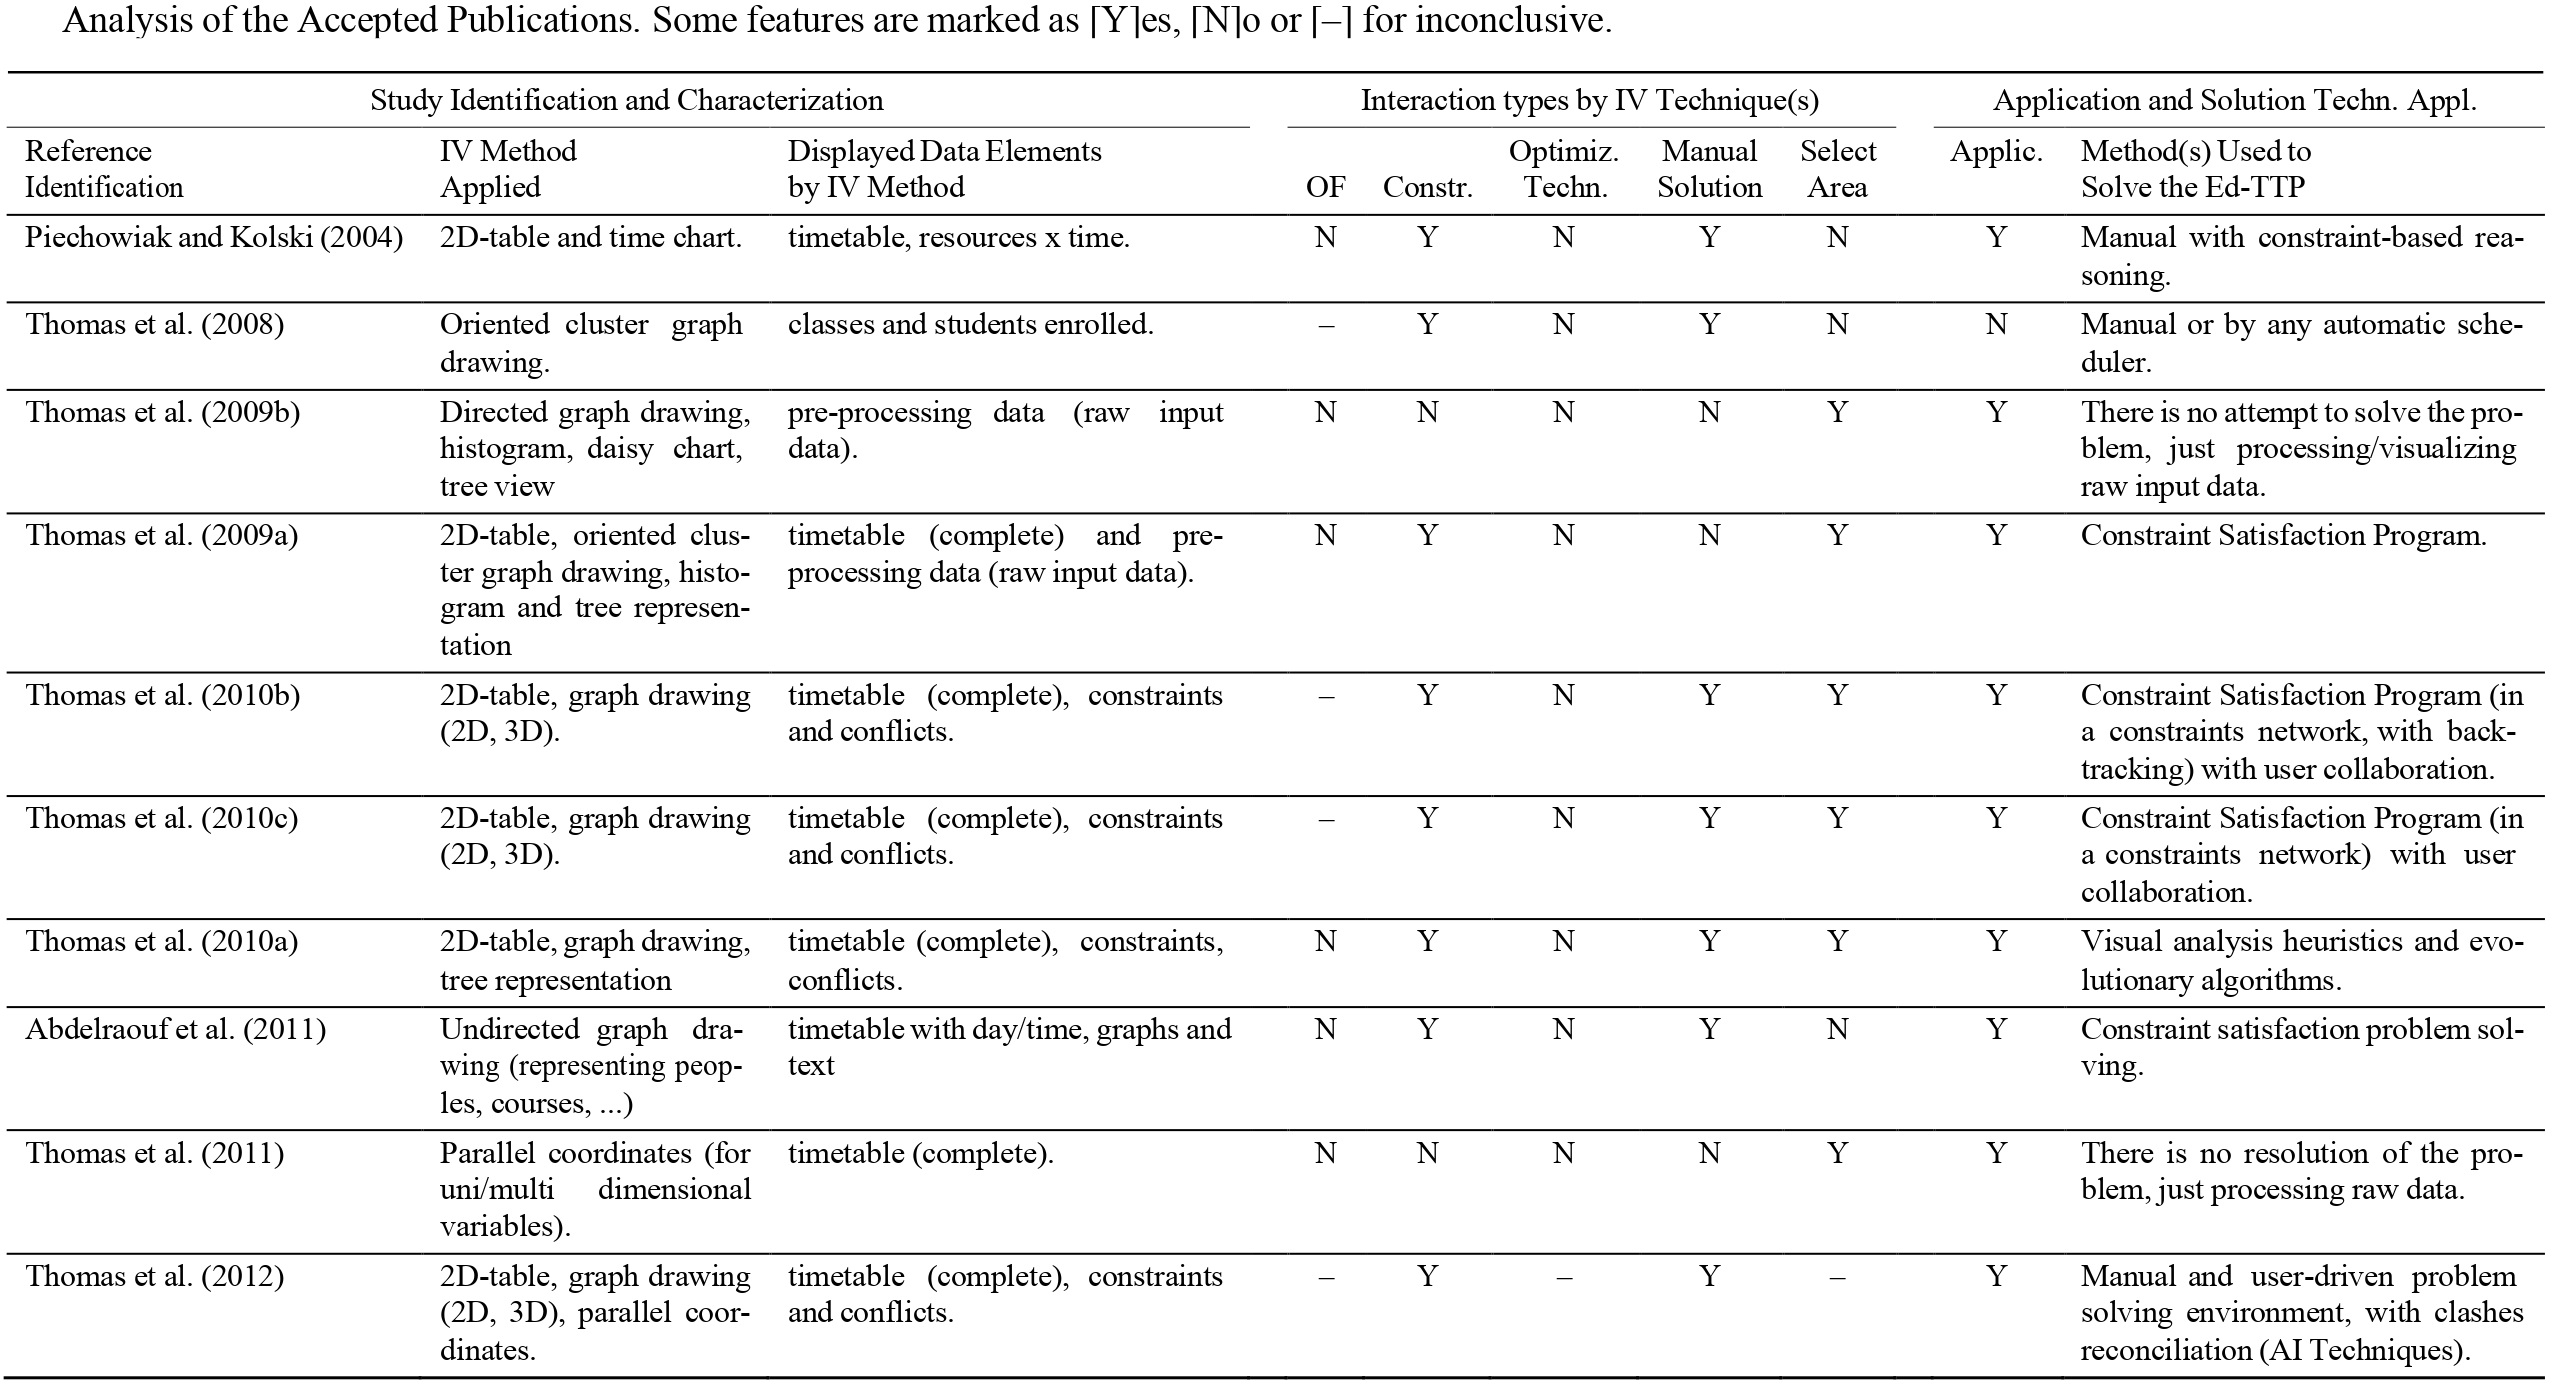
\includegraphics[width=\textwidth]{files/img/2.02!2-marco/Visualization}
  \legend{Fonte: \citeonline{Alencar2019} - editado}
\end{CenteredFigure}    % Visualization

\section{Problema de \textit{timetabling} na UENF (PTT-UENF)} \label{sec:anteriores}                               % ###  2.4

Como visto nas seções anteriores, cada instituição de ensino possui suas próprias características e particularidades. E para a UENF não é diferente. O PTT-UENF apresenta características que tornam o seu problema único, e que, portanto, necessita de uma solução específica. A instituição não se mostra desprovida de histórico na tentativa de resolução deste problema. \hyperref[ssec:sanya]{Sânya} e \hyperref[ssec:ricardo]{Ricardo}, ambos estudantes de Ciência da Computação na UENF, já realizaram trabalhos com o mesmo fim, porém com abordagens diferentes da atual proposta. Em seus trabalhos, \citeonline{SanyaSantos2013} e \citeonline{RicardoSilveira2014} abordaram a criação de tabelas horárias através de métodos de otimização, utilizando heurísticas e metaheurísticas para este fim. A seguir são descritos seus trabalhos anteriores e suas respectivas abordagens.

\subsection{Heurística construtiva para o PTT-UENF} \label{ssec:sanya}     % #### 2.4.1

Em seu trabalho, \citeonline{SanyaSantos2013} aborda o problema de Programação de Horários de Disciplinas em Universidades, tendo como foco o curso de Ciência da Computação da UENF. Sua abordagem foi a de desenvolver um software que fosse capaz de gerar uma grade horária ótima para o curso, levando em conta as restrições impostas pelo curso. Para isso, são explicados diversos métodos possíveis para se alcançar a solução desejada, passando inicialmente pelos métodos construtivos, seguido de métodos refinamento, podendo essas heurísticas serem utilizadas em conjunto com metaheurísticas. \citeonline{SanyaSantos2013} diz que ``as heurísticas são métodos aproximados que se preocupam em encontrar soluções próximas da otimalidade em um tempo computacional hábil''.

Por fim, utilizou uma heurística que consistia em respeitar uma matriz de preferência para a distribuição das disciplinas. Seguindo com o uso do \textit{Simulated Annealing} para a otimização da solução inicial.

\subsection{Metaheurísticas para o PTT-UENF} \label{ssec:ricardo}   % #### 2.4.2

Em seu trabalho, \citeonline{RicardoSilveira2014} aborda também o Problema de Programação de Horários (PPH) em instituições de ensino superior. Ele explora os diversos métodos heurísticos para resolução deste problema que visa encontrar a alocação ótima dos horários em suas grades. Ele teve como objetivo de seu trabalho a implementação de um software que fosse capaz de resolver o PPH do curso de Ciência da Computação da UENF, utilizando os métodos heurísticos Construção Gulosa e Busca Local e os métodos metaheurísticos \textit{Simulated Annealing} e Busca Tabu. Para este fim, ele utilizou a linguagem de programação C para a implementação dos métodos e a linguagem de programação Java para a implementação da interface gráfica do software. Com isso conseguiu elaborar uma ferramenta automatizada para a geração de quadros de horários, alocando aulas e professores em dias e horários disponíveis na semana.

Ele descreve também como possibilidade de trabalho futuro o aperfeiçoamento do banco de dados da ferramenta desenvolvida para que se possa armazenar mais informações pertinentes ao problema, para que o usuário possa realizar modificações no quadro de horários, sendo guiado pelo retorno do Software que informa a viabilidade da alteração, assim gerando maior flexibilidade à aplicação.

\begin{comment} % ``Não cabe muito a crítica aos TCCs anteriores não terem sido implementados''
\subsection{Modelos anteriores} \label{ssec:divergencias}           % #### 2.4.3

Ambos os trabalhos têm sido de grande valia ao rumarem na direção de uma solução para este amplo e complexo problema, percebe-se que o problema que buscaram solucionar ainda se encontra em aberto. Não tendo suas ferramentas alçado voos altos o suficiente para que se tornassem soluções definitivas para o problema no contexto da UENF.

\subsubsection*{\textbf{Sânya}} \label{sssec:sanya} % ##### 2.4.1.1

É dito por \citeonline{SanyaSantos2013} que ``[...] Como na UENF a tarefa de distribuição de sala não varia muito a cada período, sendo feito separadamente por cada centro [...]''. Embora possamos entender o conceito de ``variar muito'' como subjetivo, considerando que mesmo ao longo de um mesmo semestre existem realocações de salas e professores dentro do contexto de um mesmo Centro, podemos entender que a realidade da UENF é de fato muito dinâmica, não se encaixando completamente na solução de alocação única inicial de salas e professores.

Pode-se alegar que tratar da variabilidade de alocações de salas de um mesmo Centro foge do escopo do trabalho, porém, para que o coordenador da Computação tenha fácil acesso aos dados de alocação de salas disponíveis, faz-se necessário que seu uso esteja compartilhado com o Diretor do Centro de Ciência e Tecnologia (CCT), visto que este é o responsável pela alocação de salas de todos os cursos do CCT.

Em outro segmento ela diz que ``[...] as aulas que necessitam de salas com recursos especiais são geralmente já preestabelecidas, não há necessidade de automatizar esta tarefa de distribuição de salas'', mas a realidade é que embora algumas disciplinas tenham suas salas pré-estabelecidas, não são todas as disciplinas que possuem esta característica, isso não significa necessariamente que esta alocação é a mais adequada para a mesma. Então, todas as salas, mesmo que inicialmente pré-estabelecidas, devem estar passíveis de mudanças, mas com possibilidade de se fixar.

Ela diz também que ``Outra tarefa que no presente cenário do curso de Ciência da Computação não viabiliza algum tipo de automatização é a distribuição de professores, pois além de um número muito pequeno destes, não há muitas alternativas de mudanças de suas respectivas disciplinas.''

Quanto à distribuição de professores, a realidade do curso de Ciência da Computação segue a mesma da que foi apontada por \citeonline{SanyaSantos2013}. Entretanto, cada professor tem sua própria gama de disciplinas que se dispõe a ministrar, e a coordenação tende a distribuí-los de acordo com sua preferência. Entretanto, como a demanda dos alunos não se mostra linear como foi estudado, é possível que a distribuição de professores seja feita de forma mais eficiente, considerando a demanda dos alunos, ainda que não se descartem suas preferências pessoais.

Sânya apresenta em seu trabalho uma série de requisitos essenciais e não essenciais para a resolução do problema. Porém, alguns deles não se mostram condizentes com a realidade da universidade. São eles:

\begin{quote}\footnotesize
  \begin{itemize}
    \item Requisitos essenciais, ou seja, obrigatórios:
          \begin{itemize}
            \item \textbf{RE1} - Um professor não pode lecionar aula em duas turmas diferentes no mesmo horário.
            \item \textbf{RE2} - Uma turma não pode ter aula em duas disciplinas no mesmo horário.
          \end{itemize}
    \item Requisitos não essenciais, de qualidade:
          \begin{itemize}
            \item \textbf{RNE1} - O ideal é que existam no máximo duas aulas consecutivas da mesma disciplina.
            \item \textbf{RNE2} - Não devem haver mais de duas aulas da mesma disciplina em um dia.
            \item \textbf{RNE3} - Não preencher os horários de 12h às 14h, pois se trata de horário de almoço.
            \item \textbf{RNE4} - Os professores associados, por terem exclusividade com a instituição, preferem espalhar os horários das aulas dadas, e não acumular todas no mesmo dia.
            \item \textbf{RNE5} - Os professores contratados, por outro lado, preferem que suas aulas sejam alocadas num mesmo dia, ou no menor número de dias possíveis.
          \end{itemize}
  \end{itemize}
\end{quote}

Quanto à citada RE2, a limitação deveria ser mais criteriosa, e se tratando de um requisito não essencial, pois, o conceito de turma é dado pela junção de estudantes que cursam a mesma disciplina, ministrada por um mesmo professor, em um mesmo semestre. Mas em seu trabalho, Sânya considera o conceito de turma como sendo o conjunto de estudantes que ingressaram em um mesmo ano, independente da consideração da existência de repetentes e de suas escolhas pessoais de inscrição.

\textbf{RNE1}, \textbf{RNE2} e \textbf{RNE3}: todas elas não consideram a existência de disciplinas que necessitam de um total de cinco tempos de aula semanais, sendo elas regularmente divididas em dois períodos, um de duas horas e outro de três horas. Que, em situações de necessidades, como é visto na entrevista com o diretor do CCT, acaba sim sendo necessário que se aloque em período de almoço.

\textbf{RNE4} e \textbf{RNE5}: embora estejam direcionadas corretamente, ainda assim não engloba casos de preferência pessoal de cada um dos professores citados. Como por exemplo a possibilidade de não se ministrar aulas em determinados dias da semana por motivos religiosos, seja por parte do quadro permanente, quanto de professores associados.

Outra considerável divergência entre o modelo e a realidade é a definição de que a cada semestre contém apenas 5 turmas de computação. Sendo estas compostas pelos estudantes ingressantes de 5 anos consecutivos, caso este que não se aplica à realidade da universidade, visto que a quantidade de turmas varia de acordo com a demanda semestral, que não necessariamente condiz com todos os estudantes ingressantes de um mesmo ano.

Por fim, Sânya não considera a possibilidade de alocação de professores em mais de uma disciplina, o que é uma realidade na universidade, visto que alguns professores ministram aulas em mais de um curso, e em mais de uma disciplina.

\subsubsection*{\textbf{Ricardo}} \label{sssec:ricardo} % ##### 2.4.1.2

\citeonline{RicardoSilveira2014}, em seu trabalho, apresenta alguns conceitos que se mostraram limitantes em sua modelagem conceitual do problema na UENF. Em sua monografia, ele aborda as turmas como sendo compostas por alunos que ingressaram no mesmo ano, independente de suas escolhas, da demanda, e de possíveis defasagens na progressão do curso. O que não se mostra condizente com a realidade da universidade atualmente, então, mesmo que em 2014, quando o trabalho foi realizado, a realidade fosse esta, não se mostra condizente com a realidade atual, havendo então a necessidade de uma reformulação conceitual.

Ele, assim com \citeonline{SanyaSantos2013}, também não considera a possibilidade de alocação de professores em mais de uma disciplina, múltiplas turmas de uma mesma disciplina, assim como não lida com a distribuição das salas. Ele também considera algumas disciplinas estão fixas, mesmo que pudessem sim ser modificadas por seu responsável, o Diretor do CCT.

Por fim, podemos citar um outro ponto que é a busca pela eficiência e baixo custo de tempo dos métodos utilizados. O que se mostra como ponto positivo, entretanto, mesmo com tamanha eficiência ainda peca em atingir a praticabilidade da solução.

\subsubsection*{\textbf{Parecer geral das divergências}} \label{sssec:divergencias} % ##### 2.4.1.3

O entendimento das falhas passadas em se encontrar uma solução prática ao problema de Programação de Horários da UENF é de suma importância para que se possa evitar que os mesmos erros sejam cometidos novamente. Assim, é necessário que se tenha em mente que a realidade da universidade é dinâmica, e que a solução deve ser capaz de se adaptar a esta dinamicidade.

Vale-se também relembrar o que é dito por \citeonline{Murray2007} que citam em seu trabalho justamente sobre a complexidade presente na modelagem do problema.
\end{comment}

\subsection{Grade horária do curso de Engenharia Civil da UENF} \label{ssec:leciv}                        % #### 2.4.3

Através de pesquisas no \LinkToURL{\LinkSiteUENF}{site oficial da UENF}, mais especificamente na página de horários do LECIV para 2017.2 e 2018.2 foram encontrados alguns PDFs que continha a grade horária do curso de Engenharia Civil para o período de 2017 e 2018. A \autoref{fig:LECIV} ilustra a página referente às disciplinas do sexto período.

\begin{CenteredFigure} \caption{Grade horária do LECIV para 2017.2 e 2018.2} \label{fig:LECIV}
  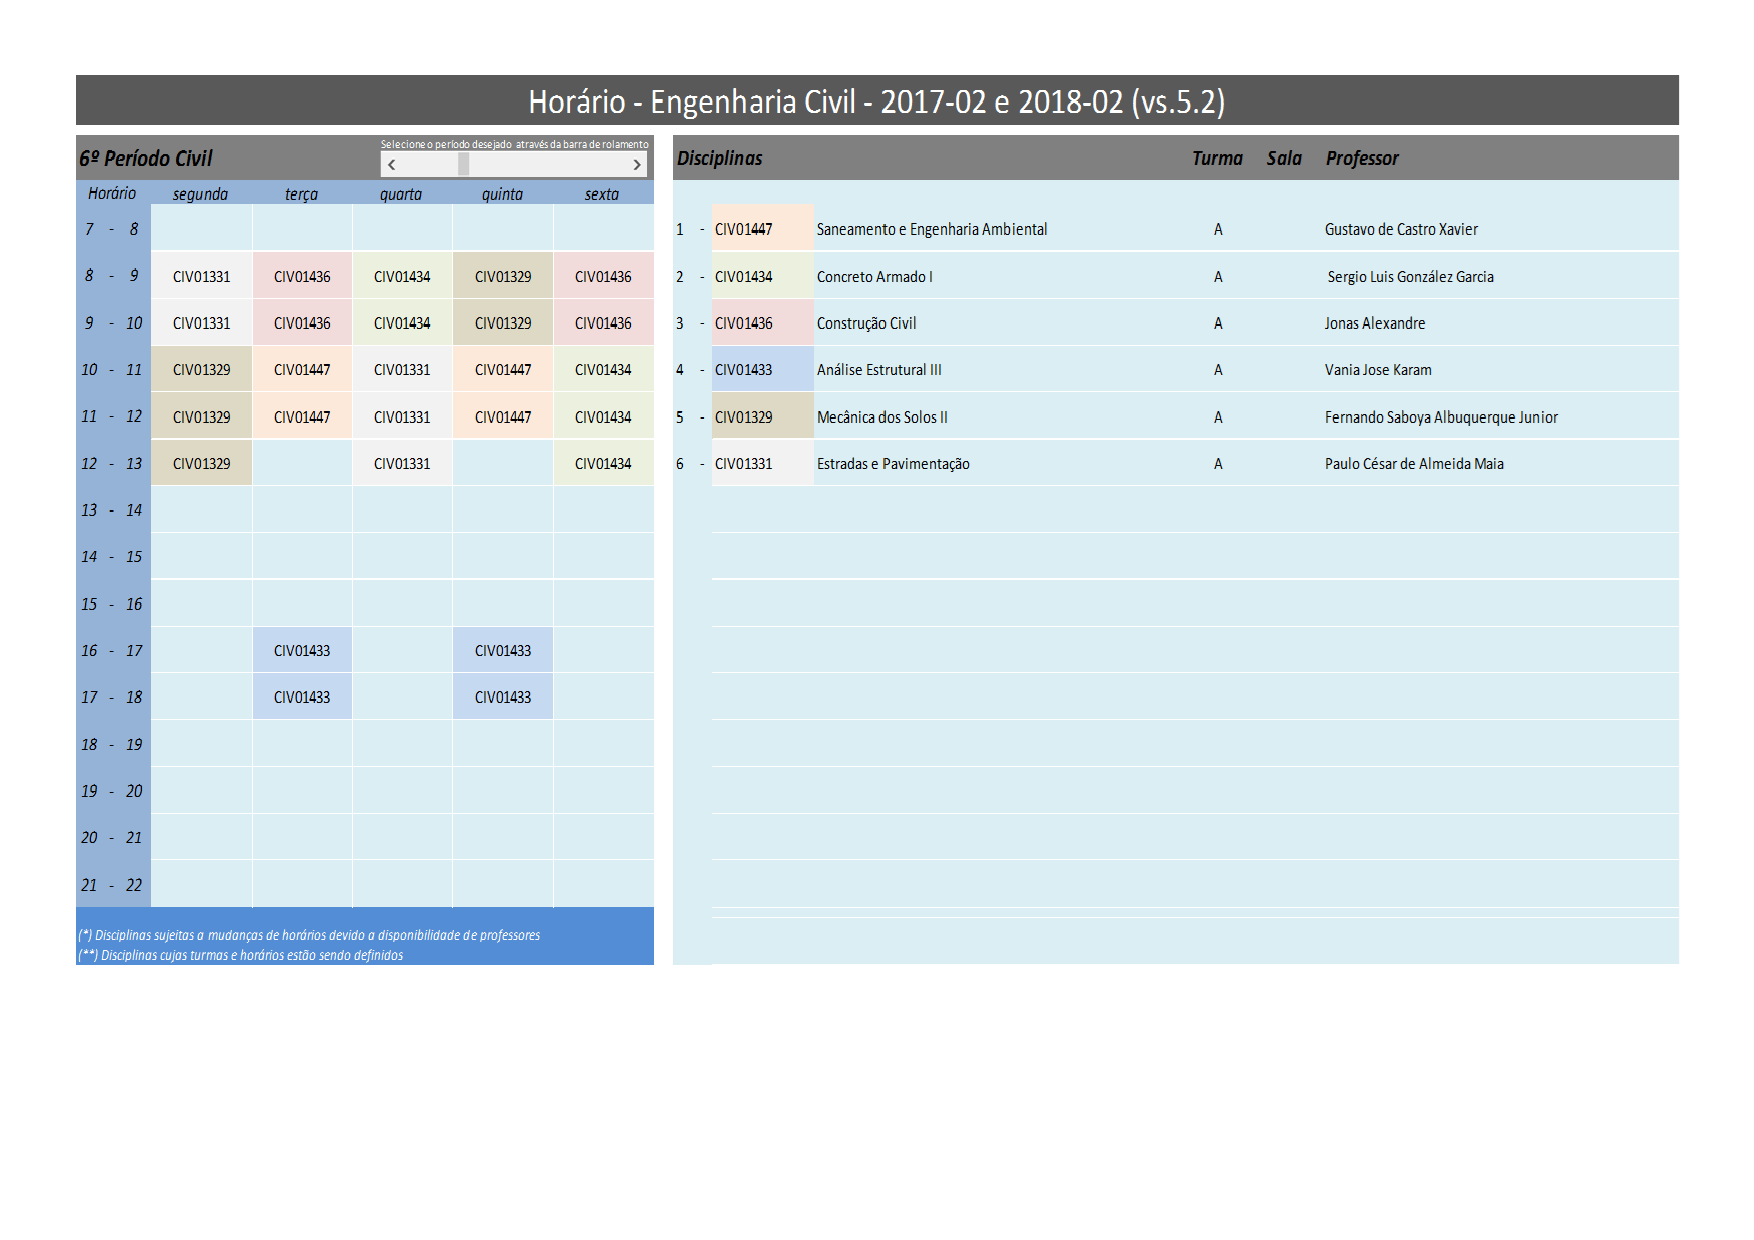
\includegraphics[width=\textwidth]{files/img/2.02!2-marco/GradeHoráriaLECIV}
  \legend{Fonte: \citeonline{Haddad2018}}
\end{CenteredFigure}

Quanto a análise desses documentos sobre esta grade algumas conclusões podem ser obtidas: 1. Esta forma de criação de grade foi mantida até no mínimo a data de 31/08/18 que consta no nome de um dos arquivos; 2. Foi utilizado o conceito de curva de nível com uma barra deslizante para visualizar a grade horária de cada período; 3. Com a legenda, entende-se que já se trabalhava com a ideia de maleabilidade de horários e também a ideia de alteração iterativa da grade; 4. Não se sabe ao certo se esta grade fora criada através de um software de criação de planilhas ou se foi criado através de um site.

Conclui-se então que esforços para se criar formas grades horárias intuitivas e maleáveis não estão limitados apenas ao curso de Ciência da Computação, também se estendendo a outros cursos da UENF.

\section{Estratégias de solução baseadas na otimização} \label{sec:teorias}                               % ###  2.5

Dentro do corrente trabalho, algumas teorias e métodos de resolução de problemas foram utilizados, sendo estes embasados por pesquisas anteriores.

\subsection{Relaxar restrições para encontrar soluções} \label{ssec:relaxar}                              % #### 2.5.1

Uma das formas de se encontrar soluções para problemas complexos é relaxando as restrições. Esse método consiste em ``permitir violações das restrições rígidas'' \cite{Dunke2023}, assim permitindo que soluções inviáveis sejam aceitas e posteriormente corrigidas.

Ao utilizar do método da programação inteira, \citeonline{Dunke2023} flexibilizam as restrições de seu modelo de programação linear, porém utilizam de uma heurística que corrige as soluções encontradas. De forma similar, \citeonline{Souza2000} menciona o uso de Algoritmos Genéticos que gera frequentemente soluções inviáveis, sendo utilizado então um filtro para que as inviabilidades sejam reparadas.

Com isso, entende-se que a flexibilização das restrições pode ser uma forma de se encontrar soluções viáveis. Ao permitir que esta categoria de soluções seja percorrida, abre-se a possibilidade de se encontrar outras soluções potencialmente viáveis que poderiam não ser encontradas de outra forma.

\subsection{Pontos de vista das dimensões do problema} \label{ssec:pontos}                                % #### 2.5.2

\citeonline{Piechowiak2004} lidam com a busca por uma solução para o problema de alocação de horários em universidades, utilizando-se de um sistema de suporte à decisão. Seu enfoque é em auxiliar o usuário em suas decisões, visando a interatividade, adaptabilidade e qualidades ergonômicas. Nele, o autor aborda a importância de se considerar que diferentes usuários têm diferentes pontos de vista e que devem cada um resolver sua parte local do problema em questão. O problema global é o \textit{design} e gestão das grades horárias de todos os recursos, entretanto, cada um dos ``gestores educacionais'' apenas veem uma parte do problema, porém, como os recursos são compartilhados, diversos conflitos acabam ocorrendo.

\subsection{Uso de soluções anteriores, soluções parciais e desvio de conflitos} \label{ssec:parciais}    % #### 2.5.3

\citeonline{Burke2000} consideram em seu trabalho o uso de casos preexistentes para que o problema encontre uma solução similar às anteriores. É visto com otimismo o uso da análise de grafos e sub-grafos como forma de se encontrar soluções parciais para o problema, pois permite a reutilização de soluções já processadas previamente. Em seu algoritmo, ao encontrar um sub-grafo similar ao problema atual, a solução é então adaptada para o problema atual. No caso da solução parcial encontrada apresentar conflitos, então as partes conflituosas são desalocadas, ordenadas da mais conflituosa pra menos conflituosa e então são realoacadas no primeiro horário viável.

\citeonline{Arratia2021, Miranda2012, Piechowiak2004, Burke2000} apontam a recorrência de instituições de ensino que utilizam as soluções anteriores como base para a criação de novas grades horárias. Pois, devido à similaridade do problema ao longo dos anos, é esperado que parte da busca por soluções seja facilitada pela reutilização de soluções anteriores.

\subsection{Informações ausentes e professores faltantes} \label{ssec:ausentes}                            % #### 2.5.4

\citeonline{Arratia2021} também citam em sua pesquisa a possibilidade de existirem turmas de determinadas disciplinas que não apresentam professores suficientes para ministrá-las. Neste caso, esta alocação é então marcada para que seja feita a distinção das demais. Assim gerando uma solução parcial para o problema, que pode ser resolvida posteriormente com a contratação de professores para ministrar as disciplinas faltantes.

\subsection{Sistemas de suporte à decisão} \label{ssec:sistemas}                                            % #### 2.5.5

O uso de sistemas de suporte à decisão é citado por \citeonline{Miranda2012} que menciona o uso de tais sistemas para o agendamento de cursos por mais de duas décadas. \citeonline{Piechowiak2004} também mencionam o termo, abordando em seu trabalho uma ferramenta de suporte a decisão que permite a alocação de horários evitando conflitos, mesmo que primeiro permita-se a existência deles, para que então sejam resolvidos. \citeonline{Frada2008} por sua vez definem o campo de Sistemas de Suporte à Decisão como ``uma disciplina aplicada que usa conhecimento e, especialmente, teoria de outras disciplinas''. Também é descrito como a forma ``como computadores e modelos analíticos podem ajudar os gerentes a tomar uma decisão-chave de planejamento de negócios recorrente'' \cite{Frada2008}.
